\documentclass[prd, nofootinbib, floatfix, 11pt,tightenlines,times]{article}

% latex W13report.tex; bibtex W13report; latex W13report; latex W13report; dvips W13report; gv W13report.ps

\usepackage[paperwidth=8.5in,paperheight=11in,centering,margin=1in]{geometry}
\usepackage{amsmath}
\usepackage{amsbsy}
\usepackage{natbib}
\usepackage{rotating}
\input epsf
\usepackage{amsmath}
\usepackage{wasysym}
\usepackage{subfigure}
\usepackage{graphicx}
\usepackage{epsfig}
\usepackage{color}
%\usepackage{ulem}
%\usepackage{epstopdf}

%\renewcommand{\baselinestretch}{0.98}
\usepackage{epsfig}
\usepackage{titletoc}

% HOW TO SET UP AN 8.5 x 11:
% http://www.pages.drexel.edu/~pyo22/students/latexRelated/latexTutorial.html
\topmargin -1.5cm        % read Lamport p.163
\oddsidemargin -0.04cm   % read Lamport p.163
\evensidemargin -0.04cm  % same as oddsidemargin but for left-hand pages
\textwidth 16.59cm
\textheight 21.94cm 
\parskip 7.2pt           % sets spacing between paragraphs
\parindent 0pt		     % sets leading space for paragraphs

\def\aap{{\it Astr.~Ap.}}     %Astronomy & Astrophysics%
\def\aaps{{\it A\&AS}}
\def\apj{{\it ApJ}}

\author{Andrew Becker, Simon Krughoff, Andrew Connolly, Russell Owen}
\title{Summary of Late Winter2013 Production: ip\_diffim}
\date{\today}

\begin{document}

\maketitle

We summarize

\clearpage
\tableofcontents
\clearpage

\section{Introduction}

The focus of this production is to ascertain the ability of the LSST
software stack to provide clean subtractions between a science image
and a reference image (referred to as the template image below).  The
science image will typically be a single--epoch {\tt calexp}, while
the template image will be a high signal--to--noise representation of
the field, typically a {\tt coadd}.

The metric we use to define ``clean'' is the number of false positives
that are detected and measured on the image difference.  We calculate
several additional quality metrics during the image subtraction
process, and correlate them with the number of false positives, as a
means to predict the number of false positives we may expect
downstream from the image subtraction itself.

\subsection{Algorithm}

We establish the math behind the process below.  

We assume that science image $S(x,y)$ can be modeled as a convolution
of the template image $T(x,y)$ by a PSF--matching kernel $K(u,v,x,y)$.
We further assume that the kernel may be decomposed using a set of
basis functions $K(u,v) = \sum_i a_i K_i(u,v)$, where the coefficients
in front of each basis are determined through:
%
\begin{eqnarray}
C_i & \equiv & (K_i \otimes T) \\ \nonumber
b_{i}  & = & \sum_{x,y} {{C_i(x,y) S(x,y)}\over{\sigma^2(x,y)}}   \nonumber \\ 
M_{ij} & = & \sum_{x,y} {{C_i(x,y) C_j(x,y)}\over{\sigma^2(x,y)}}  \nonumber \\ 
a_{i}  & = & M^{-1}_{ij} b_{j} \nonumber 
\label{eq-soln}
\end{eqnarray}
where $\sigma^2(x,y)$ is the per--pixel variance stored in the {\tt
  variance} plane of each LSST {\tt exposure}.  To generate a
spatially varying model for the kernel, we assume that the relative
weights of the basis functions $a_i$ themselves vary spatially,
i.e. $K(u,v,x,y) = \sum_i a_i(x,y) K_i(u,v)$.  The image difference is
then calculated through $D(x,y) = S(x,y) - T(x,y) \otimes K(u,v,x,y)$.

The basis functions themselves $K_i(u,v)$ are a degree of freedom in
this problem.  The original implementations \citep{Alard98,Alard00}
used a set of 3 Gaussians (represented by our {\tt Config} variable
nGauss), each with a different sigma (sigGauss), and each modified by
a Laguerre polynomial to a given order (degGauss).  Subsequent studies
\citep[e.g.][]{2007AN....328...16I} have suggested that a constant
ratio be maintained between the different Gaussian widths, such that
$\sigma_{i+1} = \beta \times \sigma_{i}$.  We use the value $\beta =
2.0$ for this production.  We normalize the sigmas by noting that,
under the assumption that the Psfs of the images are Gaussian
($\sigma_S$ for the science image and $\sigma_T$ for the template
image), the sigma of the matching kernel should be simply $\sigma_K^2
= \sigma_S^2 - \sigma_T^2$.  We use this width for the central
Gaussian in our sequence, when we use more than one Gaussian, or the
sole Gaussian in the sequence when we use only one.

Detection on the difference image occurs through correlation of
$D(x,y)$ with the science image's Psf, yielding optimally filtered
detection image $D'(x,y) = D(x,y) \circ Psf_S(x,y,u,v)$ where $\circ$
denotes correlation.  The values of the pixels in $D'(x,y)$ provide a
maximum likelihood estimate of there being a point source at that
position.  Detection occurs by simply finding pixels that are more
than N sigma above the variance.  

In this production, we investigate two orders of operations for the
optimal filtering by the Psf.  In the first, we Psf--match the
template image to a pre--filtered science image:
\begin{eqnarray}
D_{Pre}(x,y) & = & S(x,y) \circ Psf_S(x,y,u,v) - T(x,y) \otimes K(u,v,x,y) \nonumber \\ 
D'_{Pre}(x,y) & = & D_{Pre}(x,y). \nonumber 
\end{eqnarray}
By pre--smoothing the image that we are matching the template to --
$S(x,y) \circ Psf_S(x,y,u,v)$ -- we more frequently avoid the case
of psf--matching {\it deconvolution}, where the FWHM of $T$ is
narrower than $S$.  This pre--filtering increases the FWHM of the
image by $\sqrt{2}$.  The Psf matching kernels will need to be
correspondingly larger to account for the larger Psfs.  We are able to
run detection directly on this image.

In the second, which is the classical implementation of the problem,
we create a difference image that is then post--filtered with the Psf
for detection:
\begin{eqnarray}
D_{Post}(x,y) & = & S(x,y) - T(x,y) \otimes K(u,v,x,y) \nonumber \\ 
D'_{Post}(x,y) & = & D_{Post}(x,y) \circ Psf_S(x,y,u,v).  \nonumber 
\end{eqnarray}

One complication is that measurement on $D'_{Pre}$ is necessarily
different than on $D'_{Post}$.

\subsection{Implementation}

We describe the general set of classes and algorithms that are used to
undertake these operations in the LSST DM stack.  We assume that we
have the science image $S(x,y)$ as a {\tt calexp} instance as an
input.  The bounding box of the science image, in celestial
coordinates, is used to query the coadd repository to return the coadd
patches that overlap the image; this mosaiced coadd is also returned
as a {\tt calexp}.

Next, we use the DiaCatalogSourceSelector to query the ImSim reference
catalog for appropriate sources to use for Psf matching.  This
selector allows the user to specify the brightness and color range of
the objects, toggle star or galaxy selection, and to include variable
objects or not.  We select a fraction (1/5) of these objects to serve
as a control sample, in order to assess the effectiveness of
$K(u,v,x,y)$ to subtract objects that were {\it not} used in the least
squares fit.

The coadd and science {\tt calexps} are then astrometrically
registered to each other, with the resampling operations happening on
the coadd as it is expected to have larger S/N.  Object--to--object
matching, done using the source list above cross--matched with a
source list extracted from the coadd, is used to provide a relative
transformation between the two images.  RegisterTask is used to do the
astrometric resampling.  The resulting warped coadd is what we use as
the template image $T(x,y)$.  The residuals of the object--to--object
match are persisted as part of the debugging infrastructure.

Images $S(x,y)$ (optionally pre-filtered with $Psf_S(x,y,u,v)$) and
$T(x,y)$ are sent to ImagePsfMatchTask, whose purpose is to fit for
$K(u,v,x,y)$ and to produce $D(x,y)$.  The first step is to use the
Psf Gaussian sigmas to define the {\it sizes} of the Gaussians shapes
in $K_i(u,v)$.  As mentioned above, the main width is chosen to be
$\sqrt{\sigma_I^2 - \sigma_R^2}$.  We use variations on the
configuration where we use one Gaussian, with the above width, and
three Gaussians, the central of which has this width, and the others a
factor of $\beta = 2.0$ smaller and larger.  We modify each of the
Gaussians by a set of Laguerre polynomials of a given order.  The
smallest Gaussian is modified to the highest order, with the others
modified by order//2.  Figure~\ref{basis} provides an example basis
set with this configuration.  The total number of shapes in the basis
are: $\sum_i^{\rm nGauss} ({\rm degGauss}_i+1)\times({\rm
  degGauss}_i+2)/2$.  The dimensions of the Psf matching kernel are
chosen to be 6 times the largest Gaussian width, with a minimum
kernelSize of 21x21 pixels.  For kernels that are significantly
smaller than this, the Gaussians have significant (non--zero) power at
the kernel boundaries, leading to square systematic artifacts at the
scale of the kernel in the difference images.


\begin{figure}
\centering{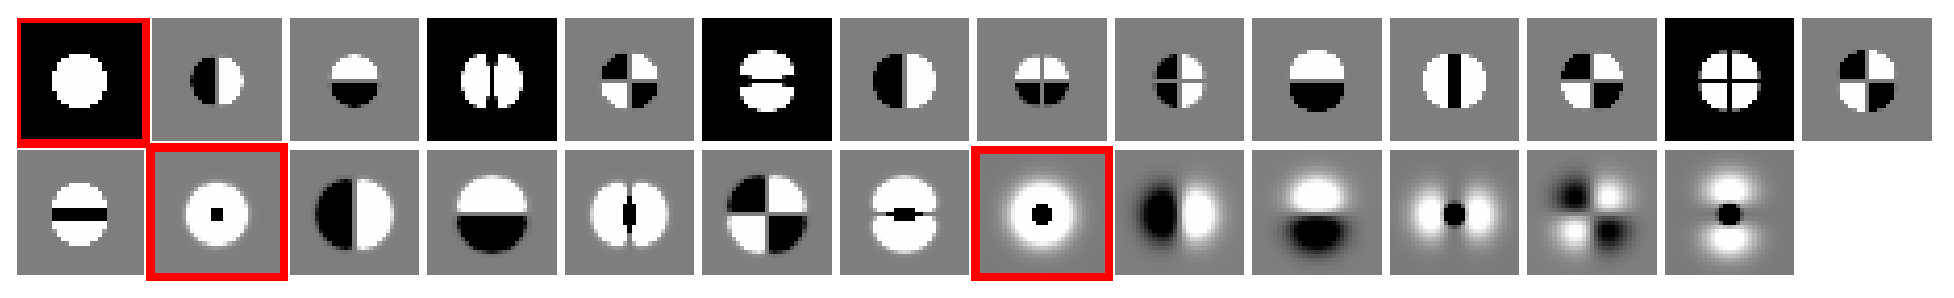
\includegraphics[width=0.8\textwidth]{figures/basis3.eps}}
\caption{Example basis set with nGauss=3 (highlighted in red),
  sigGauss=(0.5 sig, 1.0 sig, 2.0 sig), and degGauss=(4,2,2).}
\label{basis}
\end{figure}

For each source returned by DiaCatalogSourceSelector, we create a {\tt
  KernelCandidate} instance, which holds substamps of $T(x,y)$ and
$S(x,y)$ centered on the source.  These will be used to fit for a
local solution to $K(u,v)$; the ensemble of local solutions at each
source's $x,y$ will be used to fit for the full spatial solution
$K(u,v,x,y)$.  We emphasize that the dimensions of the substamps is
important.  Note from equation~\ref{eq-soln} that the coefficients
$a_i$ are derived from a convolution of the template substamp with the
kernel basis functions $K_i$.  This convolution means that
kernelSize//2 pixels along each substamp edge are rendered unusable.
To maintain a siginificant number of pixels in $C_i$, we set the
KernelCandidate dimensions to be twice that of the kernel (i.e. the
number of pixels remaining in $C_i$ is equal to the number of pixels
in the kernel, which is fewer than the number of bases $i$).


\subsubsection{ImageDifferenceTask}

The main {\tt pipeBase.Task} driving the processing is the
ImageDifferenceTask.  The calls subtasks: DiaCatalogSourceSelector;
RegisterTask; ImagePsfMatchTask; SourceDetectionTask; and
DipoleMeasurementTask.  We describe in detail each subtask below.

\subsubsection{DiaCatalogSourceSelector}

This class queries the reference catalog for {\tt sources} within the
science {\tt exposure's} footprint.  These {\tt sources are used to
  define a set of {\tt KernelCandidates} used to fit the $K(u,v)$,
  each at its specific $x,y$ coordinate.  

\subsubsection{RegisterTask}

\subsubsection{ImagePsfMatchTask}

\subsubsection{SourceDetectionTask}

\subsubsection{DipoleMeasurementTask}



\subsubsection{Configs}



\subsection{Simulations}


We use the ImageDiffereceTask to


\section{KernelCandidate Statistics}

\subsection{Mean Squared Error}

In order to investigate the bias--variance trade--off in the overall
fit, we calculate the MSE of each KernelCandidate's difference image
derived from the evaluation of the spatial model at that location.  We
define the bias as $\left| data - model \right|$, the variance as
$\left| (data - model)^2 \right|$, and the MSE as {\tt bias$^2$ +
  variance}.  In this context, the bias is the mean of the difference
image, and the variance is the mean square of the difference image.
In both cases, we normalize by the square root of the variance so that
pixels are in units of sigma.

\subsection{Reduced $\chi^2$}

\section{Dependencies of False Positive Rate}

After finding the configurations that yielded the minimal numbers of
false positives, we then perturbed the solutions to examine how the
numbers of false positives scaled with different effects.  This
included, in order of importance for this production: the difference
image detection threshold; the number of KernelCandidates going into
the spatial model; and astrometric registration errors.

\subsection{Detection Threshold}

\subsection{Number of KernelCandidates}

\subsection{Registration Errors}

We implemented two simple perturbations of the inputs to the
image--to--image RegisterTask: we first added a random offset to each
object's (x,y)-coordinates, with an amplitude that was specified in
the Config and multiplied by a random number pulled from a normal
distribution; and we added a DC offset to the coordinates at an
amplitude specified in the Config.  These offsets, added to the Source
coordinates, will affect misalignments of the objects in the
registered images, as the registration is done assuming the specified
positions are correct.  In this way we are able to investigate how
random uncertainties and bulk astrometric offsets impact the false
positive rate.  We explicitly do {\it not} investigate spatial
variation in these offsets, using for example a pincushion distortion.
We anticipate that this latter effect will be most important for
spatial interpolation and extrapolation of the matching kernel,
yielding a dipole residual field associated with the distortion.
However, the ability of the software to model out these spatial
distortions will certainly fail if the local kernel solutions (from
which the spatial model is derived) are unable to compensate for
misalignments.

\begin{figure}
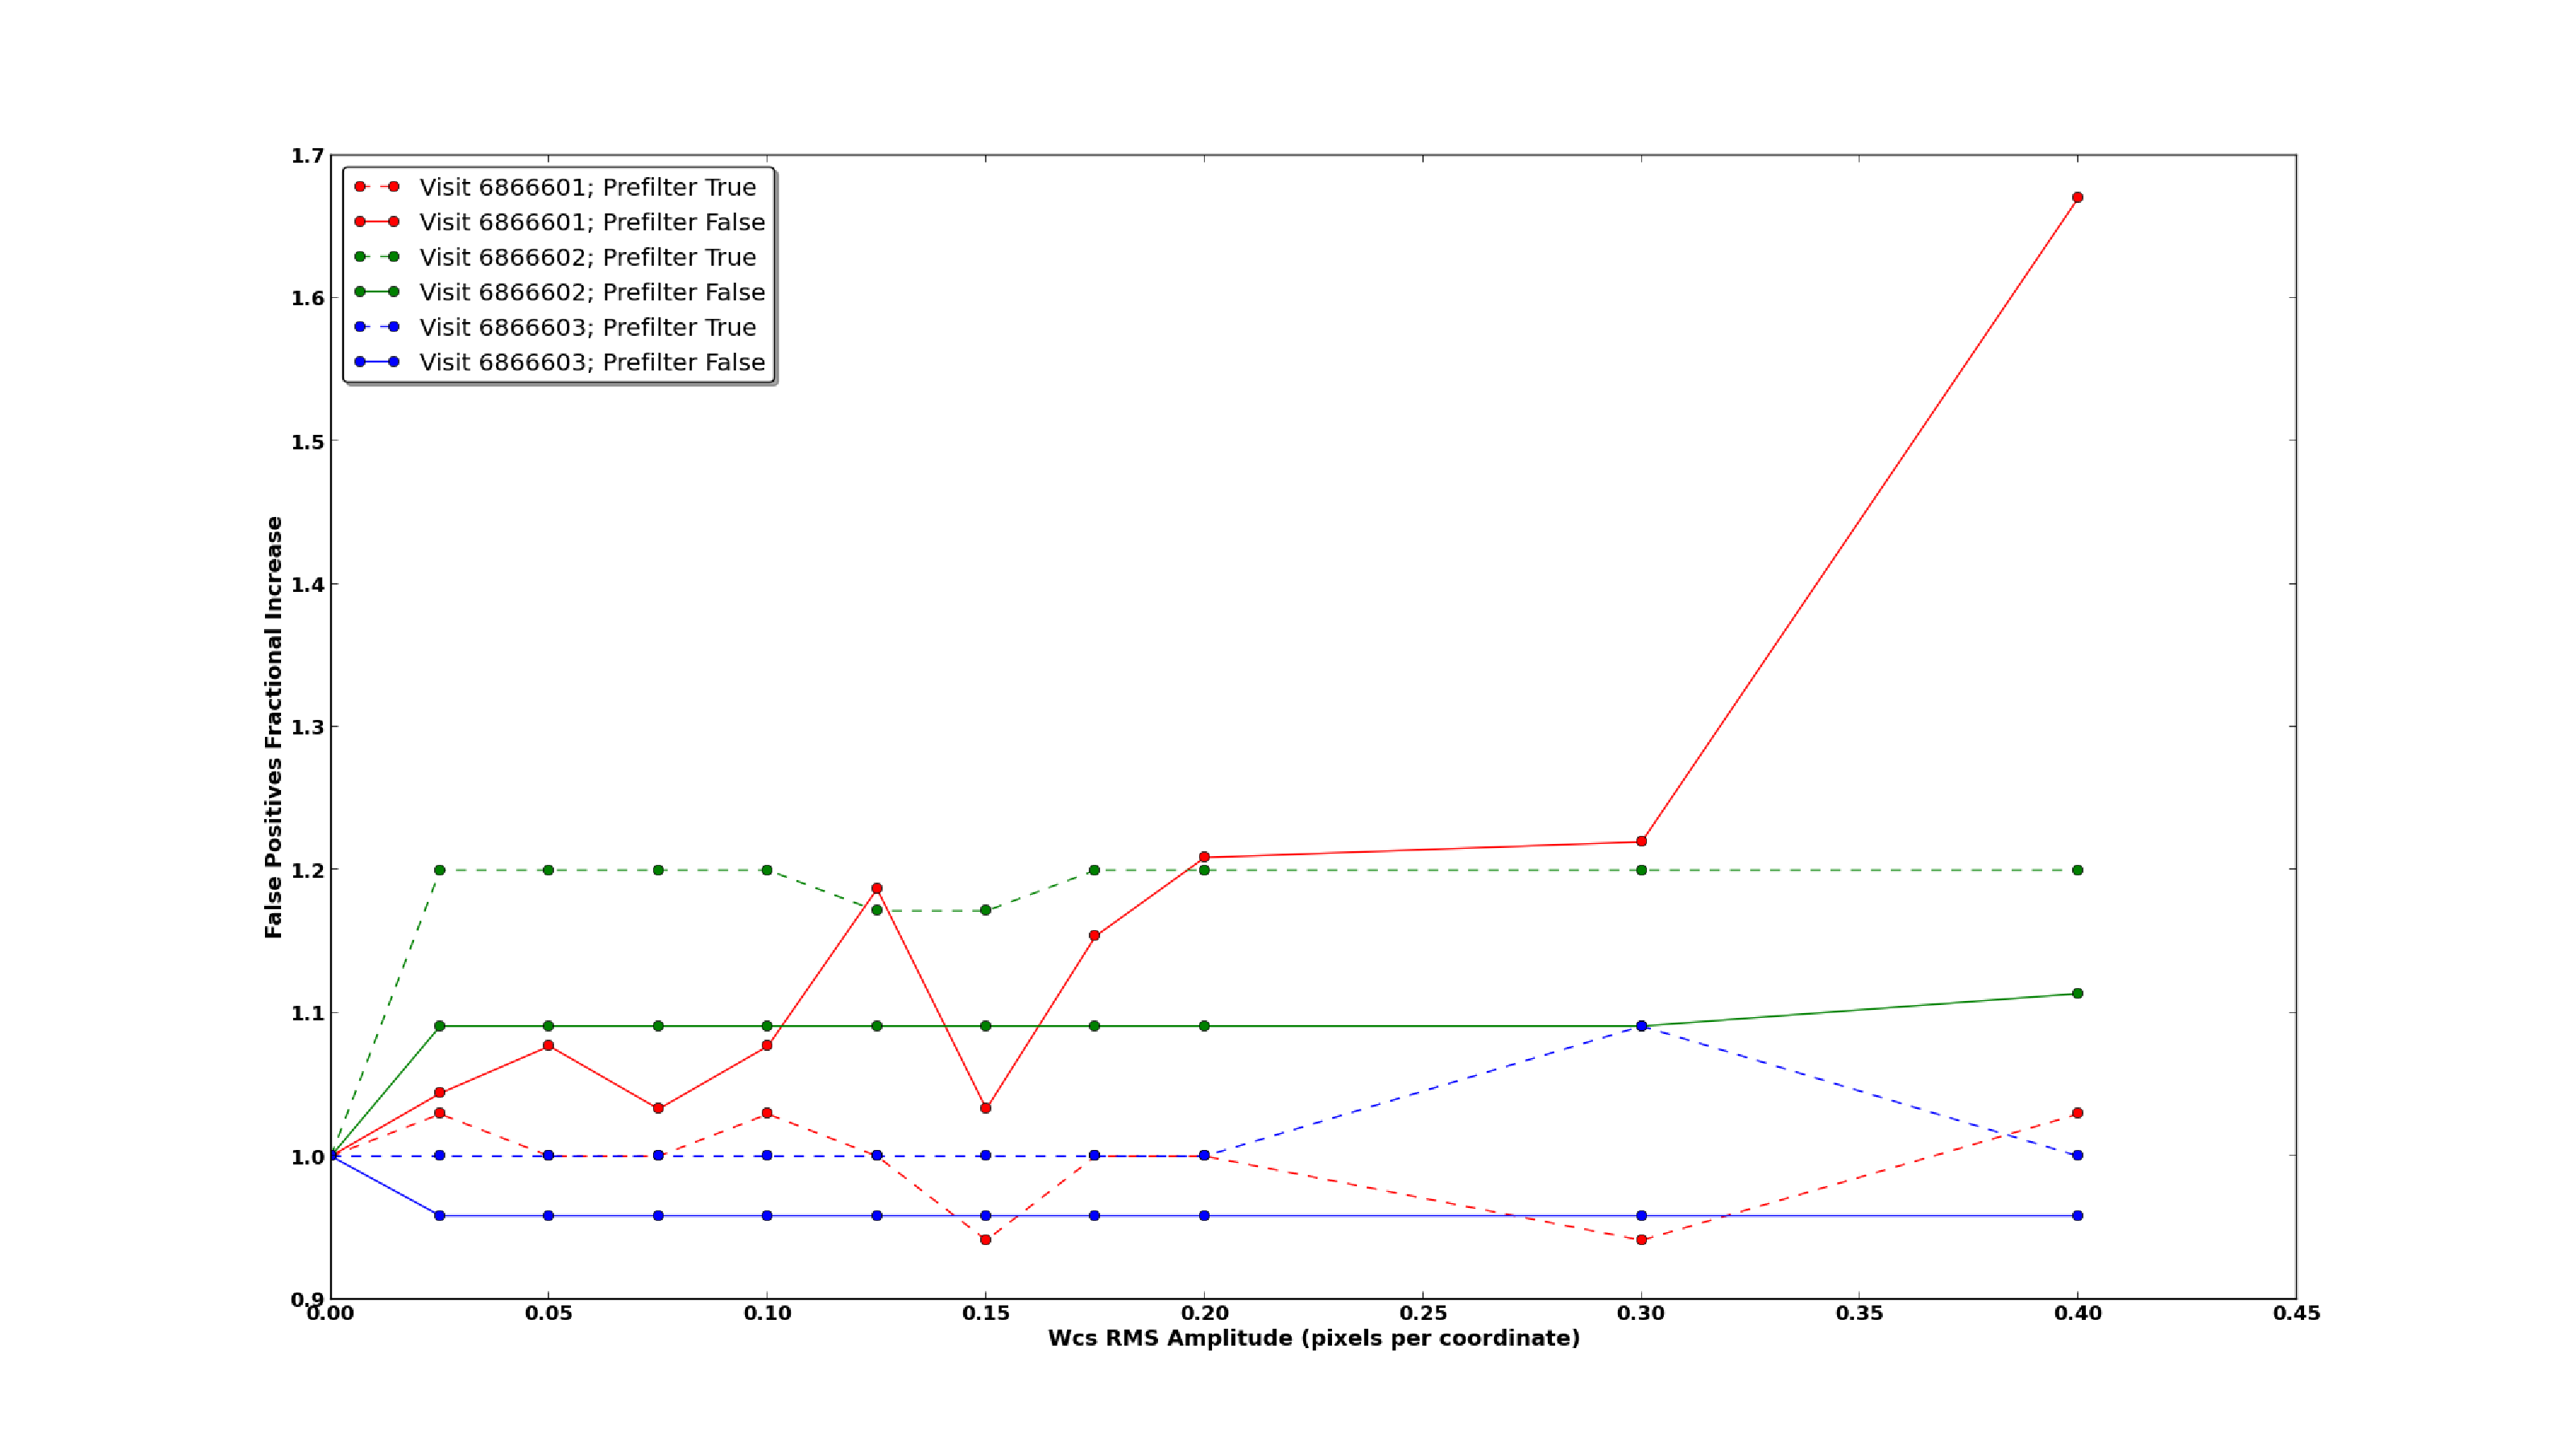
\includegraphics[width=0.5\textwidth]{figures/wcs_rms.eps} 
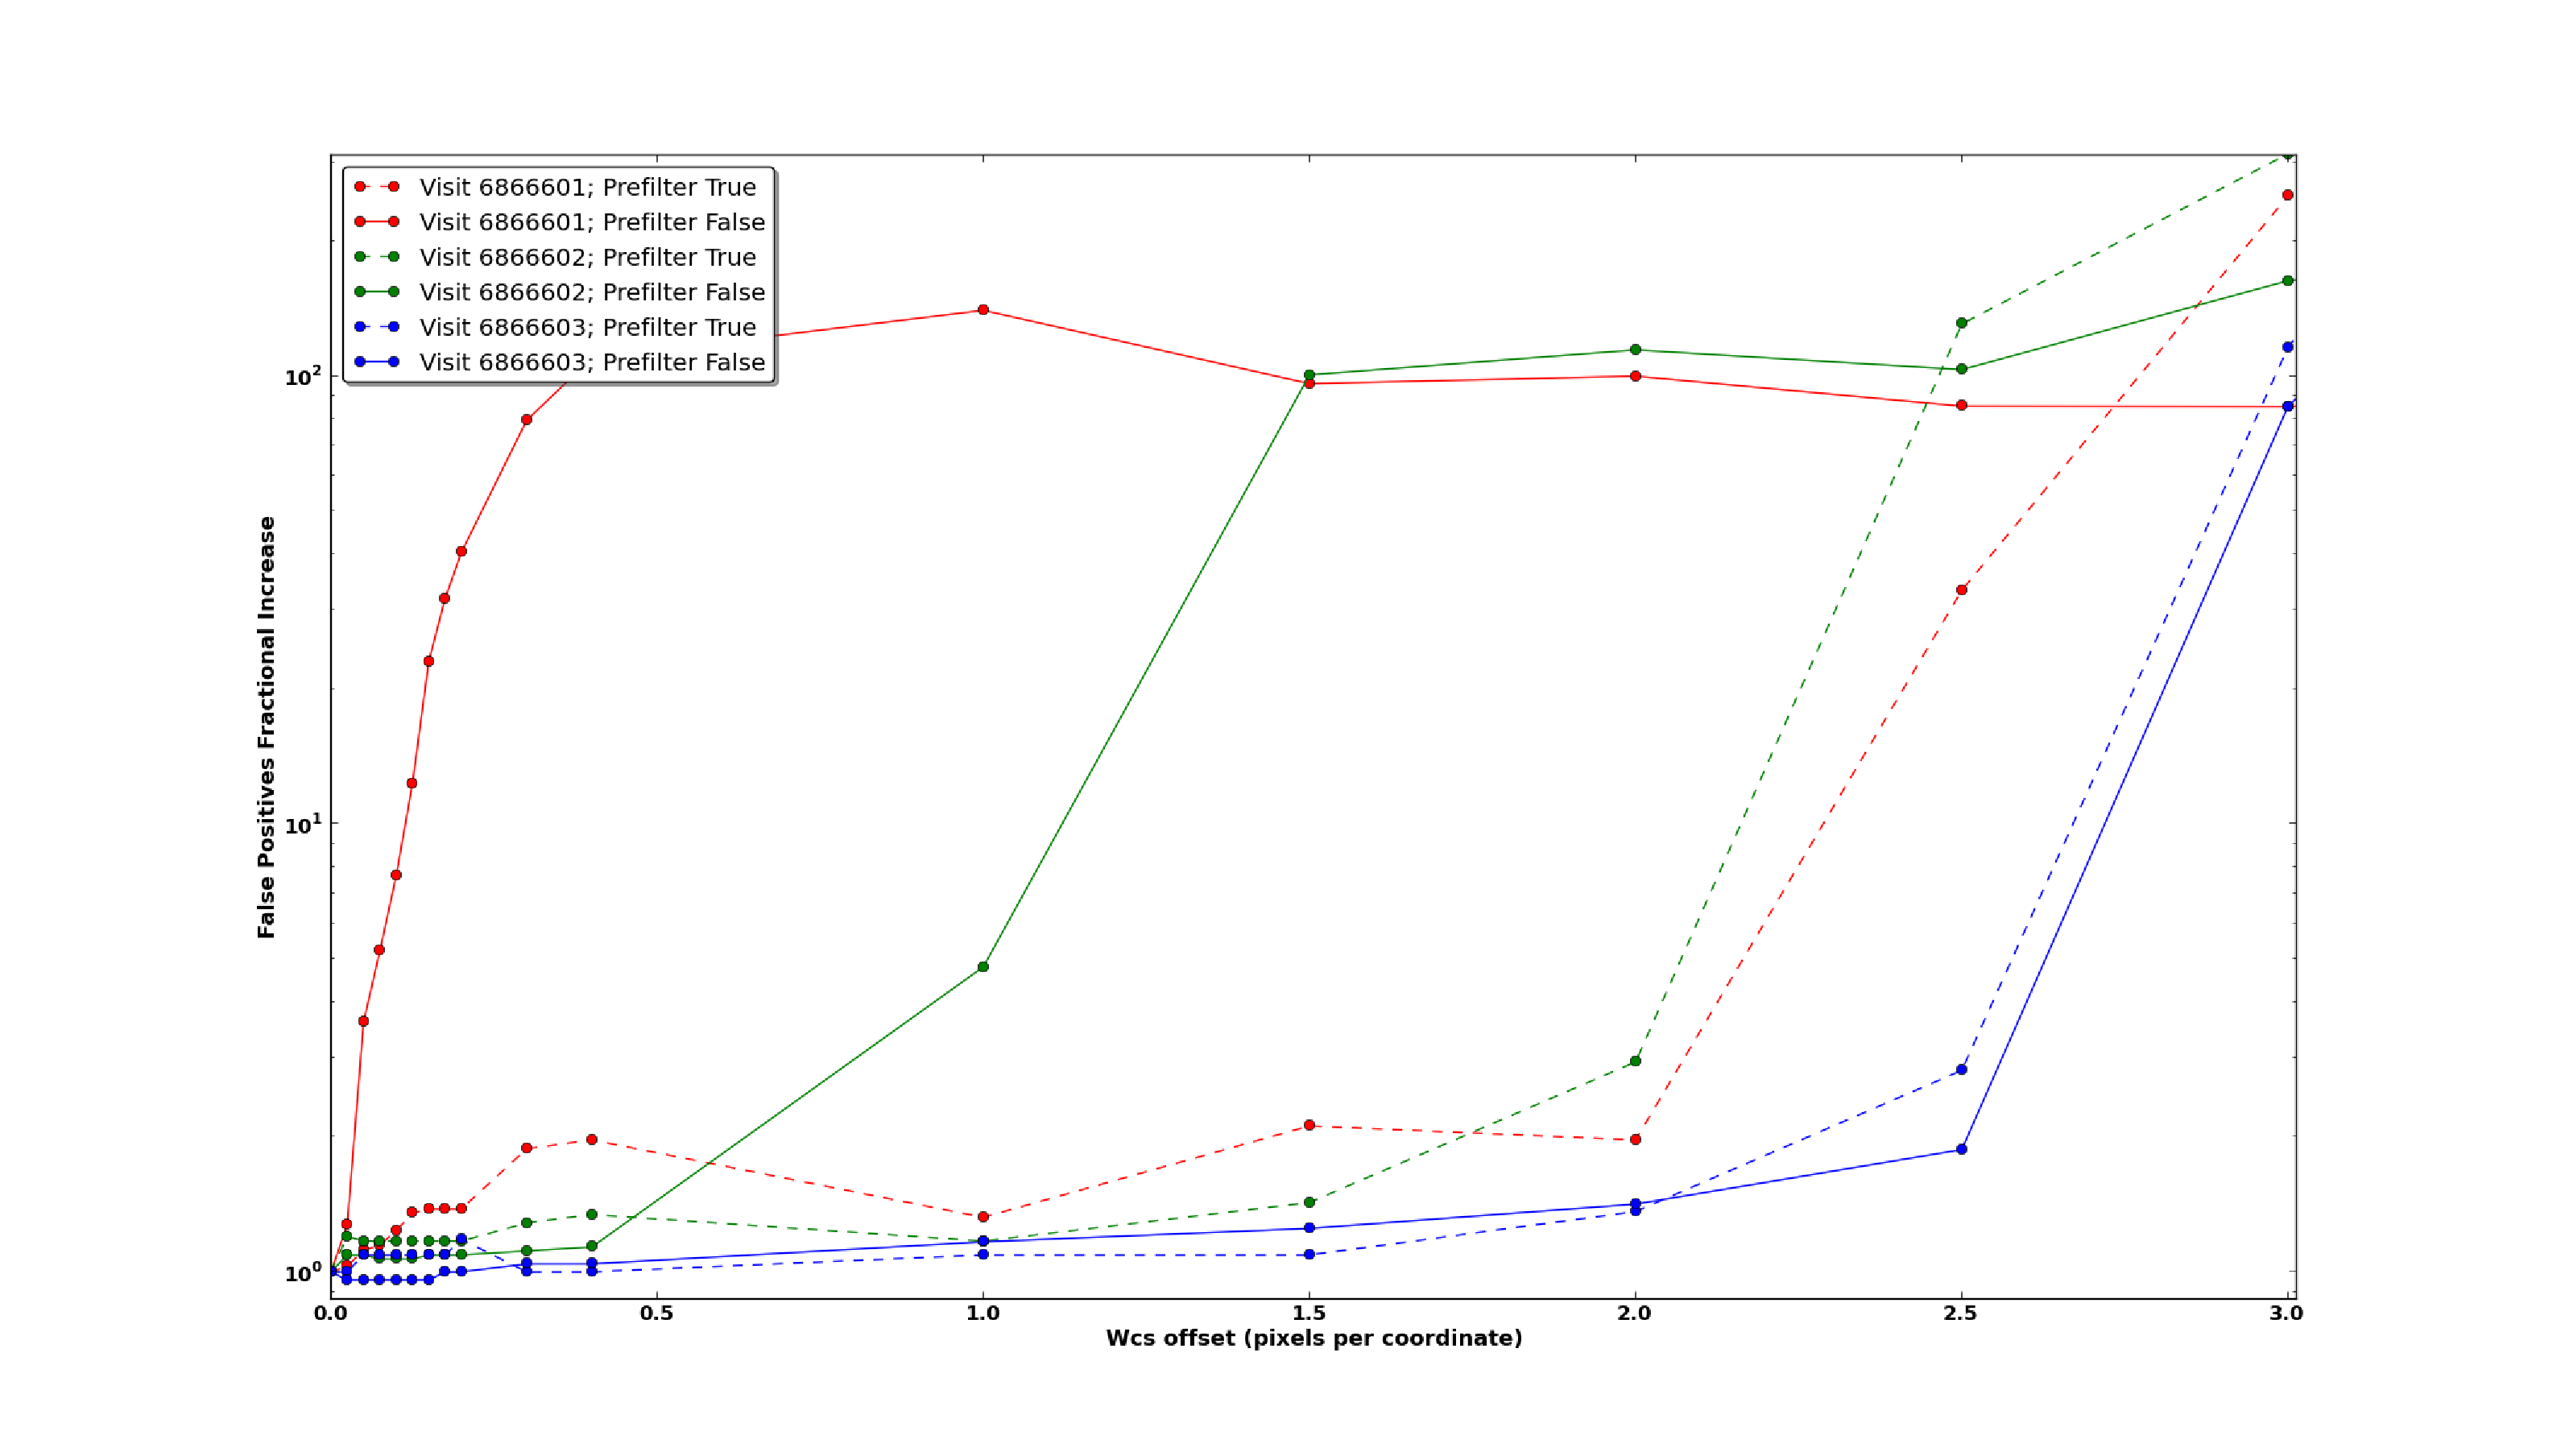
\includegraphics[width=0.5\textwidth]{figures/wcs_offset.eps} \\
\caption{WCS}
\label{wcs_offsets}
\end{figure}

\subsubsection{Coordinate RMS}

We perturbed the coordinates of each template Source that was input to
RegisterTask with amplitudes of (0.025, 0.05, 0.075, 0.1, 0.125, 0.15,
0.175, 0.2, 0.3, 0.4) pixels, and to randomize the effects we
multiplied each offset by a number pulled from a normal (0,1)
distribution.  The output RMS reported by RegisterTask was noted to
track these offsets.

The false positive rate was not seen to vary significantly.

\subsubsection{Coordinate Offsets}

We offset the coordinates of each template Source that was input to
RegisterTask with amplitudes of (0.025, 0.05, 0.075, 0.1, 0.125, 0.15,
0.175, 0.2, 0.3, 0.4, 1.0, 1.5, 2.0, 2.5, 3.0, 3.5, 4.0) pixels.
Post--registration, this will offset the positions of sources in the
two images by the desired amount.



\begin{figure}
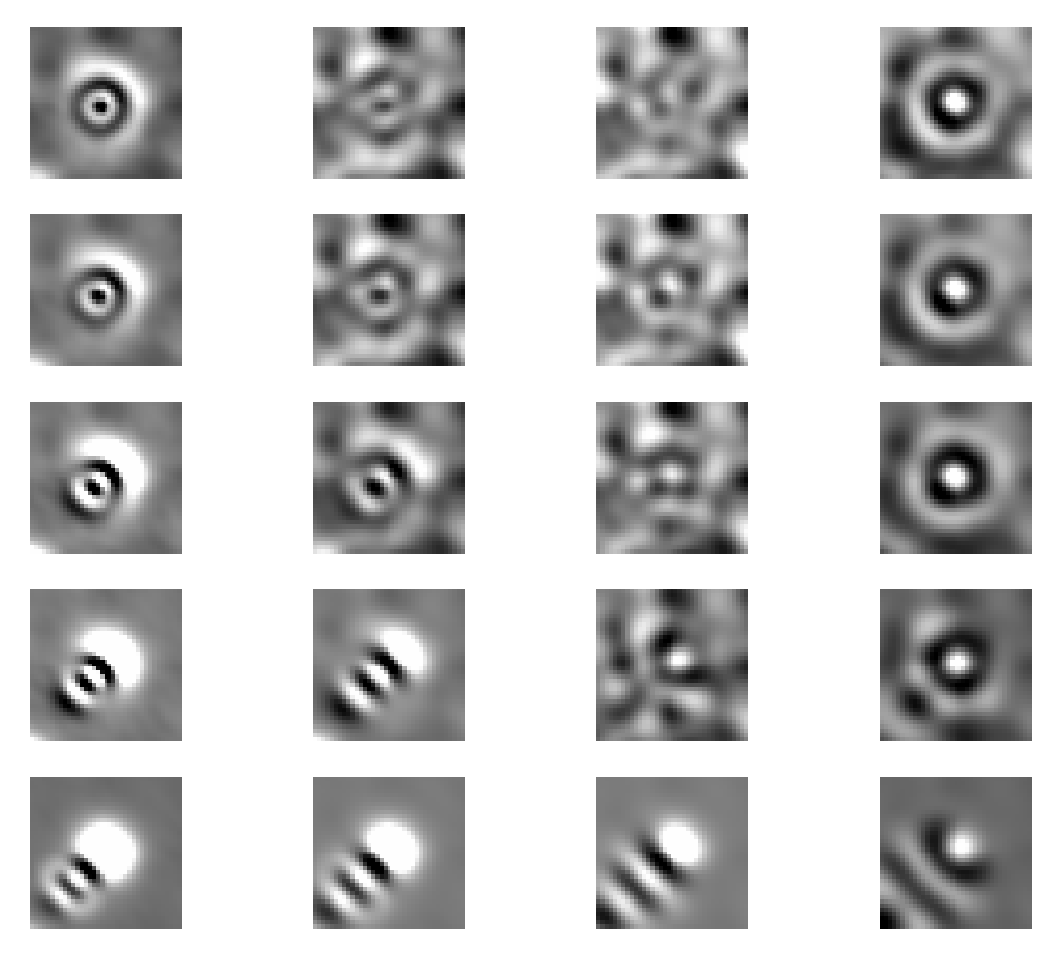
\includegraphics[width=0.8\textwidth]{figures/shift.eps} \\
\caption{Figure illustrating the ability of the kernel basis to
  compensate, locally, for the effects of misregistration.  Each
  element of the grid shows a single KernelCandidate local difference
  image (visit=6866603, doPreFilter=True).  Columns indicate the
  Gaussian sigma of the basis, which is designed to have one Gaussian
  with the prescribed width, modified to fourth order.  Rows indicate
  the amplitude of the astrometric offset that was introduced into
  the Source positions before image-to-image registration.  
  In the {\it top} row, we see that even with a small astrometric
  offset, the sigma=2 basis is unable to produce a quality
  subtraction, because the width is inappropriate for matching the two
  input Psfs (the theoretical Gaussian sigma here is 3.4 pixels).  At
  sigma=4 the basis is able to produce a quality subtraction, and by
  sigma=5 the basis is too large to match the Psfs.  In {\it row 4},
  we show that even for an astrometric offset of 4 pixels (0.8''), the
  sigma=4 basis can produce a reasonable difference image without
  structured residuals.  However, by {\it row 5}, with an offset of 6
  pixels, none of the Gaussians provide a successful local difference
  image. 
  The ability of the basis to compensate for bulk astrometric offsets
  is a function of the kernel width, and the kernel width is itself a
  function of the two input Psf FWHMs.  Thus there is a complicated
  dependence of the ability of the kernel to shift the centroids of
  stars.  Roughly, the basis may compensate for local astrometric residuals
  at a scale up to $\sqrt{\sigma_I^2 - \sigma_R^2}$.
}
\label{kernel_offsets}
\end{figure}

\bibliographystyle{apj}
\bibliography{refs}

\end{document}
